\chapter{卷积层}

\section{卷积层的特点}
	
	全连接层存在什么问题呢?那就是数据的形状被“忽视”了。比如,输入数据是图像时,图像通常是高、长、通道方向上的3维形状。但是,向全连接层输入时,需要将3维数据拉平为1维数据。全连接层会忽视形状,将全部的输入数据作为相同的神经元(同一维度的神经元)处理,所以无法利用与形状相关的信息。
	
	而卷积层可以保持形状不变。当输入数据是图像时,卷积层会以3维数据的形式接收输入数据,并同样以3维数据的形式输出至下一层。因此在CNN中,可以(有可能)正确理解图像等具有形状的数据。
	
	CNN中,有时将卷积层的输入输出数据称为特征图(feature map)。其中,卷积层的输入数据称为输入特征图(input feature map),输出数据称为输出特征图(output feature map)\cite{RN1}。

\section{卷积运算}
	
	卷积层进行的处理就是卷积运算。卷积运算相当于图像处理中的“滤波器运算”。
	
	“卷积是一种特殊的加权求和”。
	\subsection{一维离散卷积}
		\subsubsection{引入——多项式乘法}
		
		设多项式:
		\begin{equation}
			\label{eq:1}
			P\left(x\right) = a_n x^n + a_{n-1} x^{n+1} + \cdots + a_1 x + a_0
		\end{equation}
	
		\begin{equation}
			\label{eq:2}
			Q\left(x\right) = b_m x^m + b_{m-1} b^{m+1} + \cdots + b_1 x + b_0
		\end{equation}
	
		那么,
		
		\begin{equation}
			\begin{aligned}
			R\left(x\right) &= P\left(x\right) \times Q\left(x\right) \\
			& = \left( \sum_{i=0}^{n} a_i x^i\right) \cdot \left( \sum_{i=0}^{m} b_i x^i\right) \\
			& = \sum_{i=0}^{m+n} c_i x^i \\
			where, \quad c_i & = \sum_k a_k b_{i-k}
			\end{aligned}
		\end{equation}
		
		接下来,我们以 $P\left(x\right) = x^4 -x^3 +2x -4$, $Q\left(x\right) = x^2 -2x +2$ 为例。其计算结果为:$$R\left(x\right) = x^6 -3x^5 + 4x^4 -8x^2+12x-8$$
		
		其乘法的直观表示如图所示:
		\begin{figure}[!htbp]
			\centering
			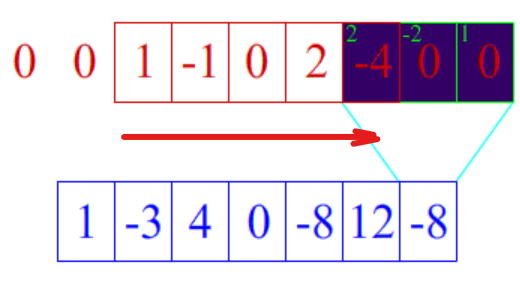
\includegraphics[width=0.50\textwidth]{conv_1}
			\caption{乘法的直观表示}
			\label{fig:1}
		\end{figure}
		
		在图\ref{fig:1}中,需要注意$Q\left(x\right)$的系数是反转哒。
		
		\subsubsection{一维离散卷积的定义}
		\begin{definition}
			如果$\left\{a_n\right\}$ $\left\{b_m\right\}$ 是两个数列, 那么二者的卷积为:
			$$c_i = \left(a * b\right) _i = \sum_k a_k b_{i-k}$$
			其中,$\left\{a_n\right\}$ 是被卷积数列, $\left\{b_m\right\}$是卷积核。
		\end{definition}
	
		在上面的例子中,如果下标不合法,则用0来代替——这是完全补0的卷积,也叫\textbf{Full卷积}。类似的,我们也可以定义如图\ref{fig:2}所示的合法卷积,也叫\textbf{Valid卷积}。
		
		\begin{figure}[!htbp]
			\centering
			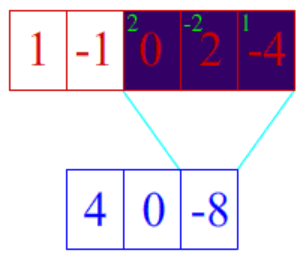
\includegraphics[width=0.30\textwidth]{conv_2}
			\caption{Valid Convolution}
			\label{fig:2}
		\end{figure}
	
		同样的,我们也可以定义\textbf{Same卷积}——卷积后的数列长度和被卷积数列一样长。具体操作仅仅比Full卷积左右各少补一半的0就可以了。
		
		在此基础上,卷积核并不一定是在被卷积数列上一格一格地滑动,可以两格两格,甚至半格半格地滑动,由此派生出无数种可能\cite{RN2}。
	\subsection{一维连续卷积}
		
		上文中涉及到的都是离散的数列,如果改为连续函数$f\left(x\right)$ 与 $g\left(x\right)$ 的卷积,那么:
        \begin{equation}
            h\left(x\right) = \left( f*g \right) \left(x\right) = \int {f\left(\tau \right) g\left(x-\tau \right)d\tau}
            \label{eq:3}
        \end{equation}
        下面我们举一个具体的例子。
        
        假设你是一个算法工程师,过着996的死亡生活,每天除了调参就是调参。你每天工作效率关于时间$t$的函数为$f\left(t\right)$ (显然,如果你准时上班,正点下班,那么$f\left(t\right) $在 $\left[0,9\right) \bigcup \left[ 21,24 \right)$ 上是没有定义的)。并且工作成果的产出关于时间$t$的函数为$g\left(x\right)$,那么你忙活一天,给团队获得的实际收益则是: 
        $$ h\left(24\right) = \int_{9}^{21} {f\left(\tau \right) g\left(24-\tau \right)d\tau} $$
    \subsection{二维离散卷积}
        上述的卷积都是一维的卷积核在一维的被卷积张量上滑动。如果被卷积张量和卷积核是二维、三维,甚至四维及以上,我们同样也可以有相同的定义——向这些维度分别滑动,分别做卷积,最后求和即可。
        \subsubsection{二维离散卷积}
        
        \begin{figure}[!htbp]
            \centering
            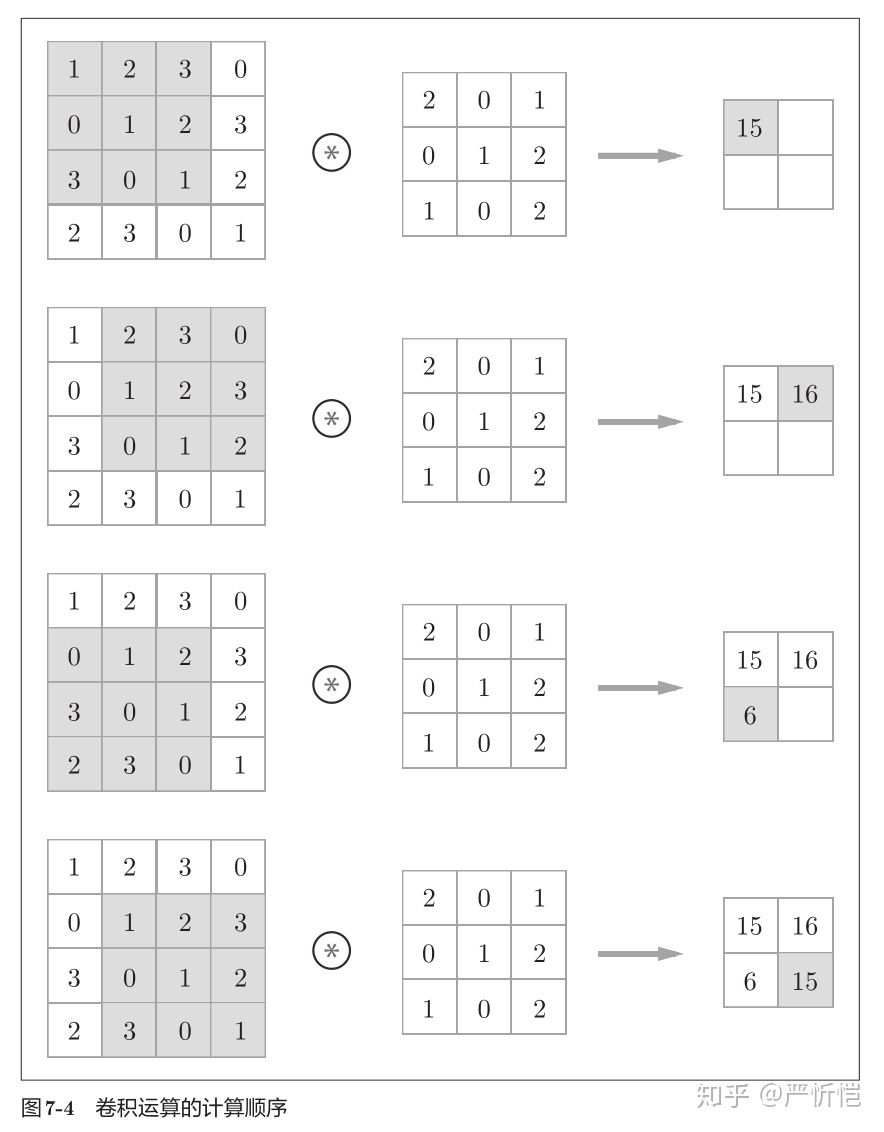
\includegraphics[width=0.90\textwidth]{conv_3}
            \caption{二维离散Valid卷积}
            \label{fig:3}
        \end{figure}
    
        \textbf{Valid卷积} \quad 如图\ref{fig:3}所示,将各个位置上滤波器的元素和输入的对应元素相乘,然后再求和(有时将这个计算称为乘积累加运算)。然后,将这个结果保存到输出的对应位置。将这个过程在所有位置都进行一遍,就可以得到卷积运算的输出。
        
    
        \textbf{Full卷积} \quad 如图所示。
      
        \begin{figure}
            \centering
            \animategraphics[width=\linewidth, autoplay=True, loop=True]{10}{Img/conv_4/conv3-}{0}{35}
            \caption{二维离散Full卷积}
            \label{fig:4}
        \end{figure}
    
        \subsubsection{偏置}
        
        有些时候,在全连接的神经网络中,除了权重参数,还存在偏置。包含偏置的卷积运算的处理流如图\ref{fig:5}所示。
        
        \begin{figure}[!htbp]
            \centering
            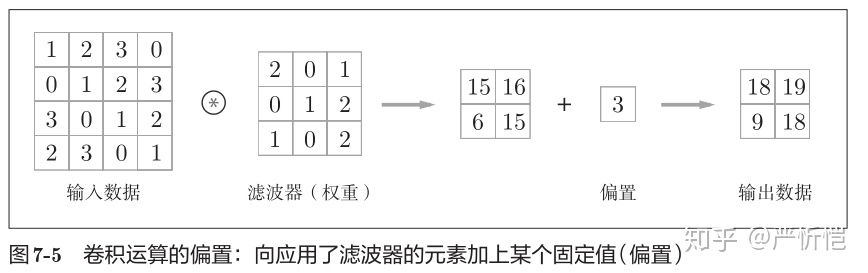
\includegraphics[width=0.90\textwidth]{conv_5}
            \caption{卷积运算中的偏置}
            \label{fig:5}
        \end{figure}
    
        \subsubsection{填充(Padding)}
        
        在进行卷积层的处理之前,有时要向输入数据的周围填入固定的数据(比如0等),这称为填充,是卷积运算中经常会用到的处理。如图\ref{fig:6}所示。
        
        \begin{figure}[!htbp]
            \centering
            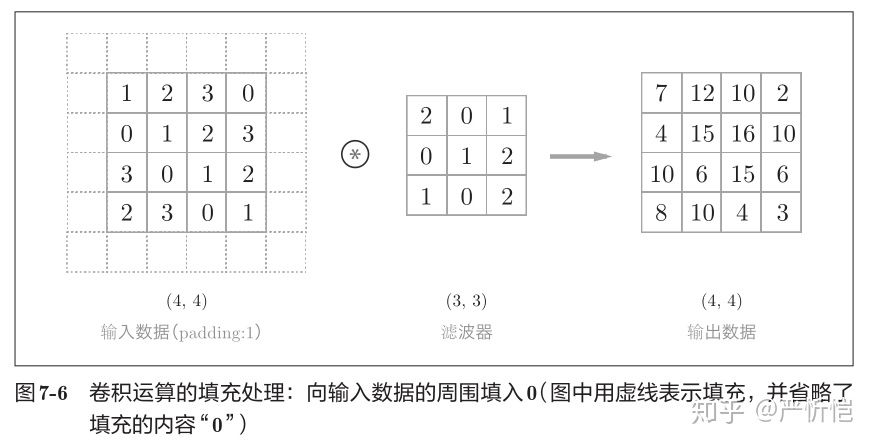
\includegraphics[width=0.90\textwidth]{conv_6}
            \caption{卷积运算中的填充}
            \label{fig:6}
        \end{figure}
    
        从图中可以看出,通过填充,大小为$(4, 4)$的输入数据变成了$(6, 6)$的形状。然后,应用大小为$(3, 3)$的滤波器,生成了大小为$(4, 4)$的输出数据。
        
        使用填充主要是为了调整输出的大小。比如,对大小为$(4, 4)$的输入数据应用$(3, 3)$的滤波器时,输出大小变为$(2, 2)$,相当于输出大小比输入大小缩小了2个元素。如果每次进行卷积运算都会缩小空间,那么在某个时刻输出大小就有可能变为1,导致无法再应用卷积运算。为了避免出现这样的情况,就要使用填充。
        
        \subsubsection{步幅(stride)}
        
        应用滤波器的位置间隔称为步幅(stride)。之前的例子中步幅都是1,如果将步幅设为2,则如图\ref{fig:7}所示,应用滤波器的窗口的间隔变为2个元素。
        
        \begin{figure}[!htbp]
            \centering
            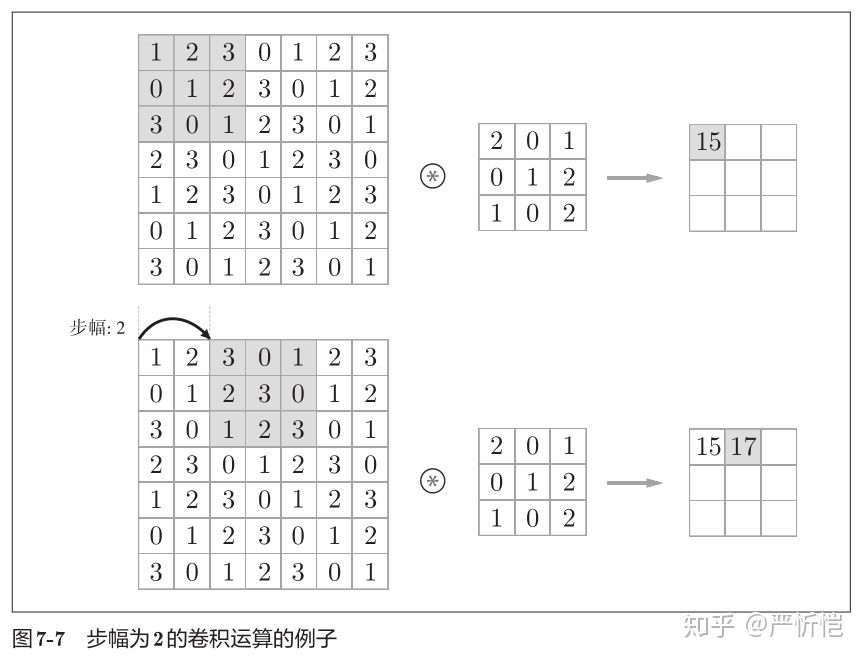
\includegraphics[width=0.90\textwidth]{conv_7}
            \caption{步幅为2的卷积运算}
            \label{fig:7}
        \end{figure}
    
        如图,对输入大小为$(7, 7)$的数据,以步幅2应用了滤波器。通过将步幅设为2,输出大小变为$(3, 3)$。
        
        综上,\uwave{增大步幅后,输出大小会变小。而增大填充后,输出大小会变大}。
        
        \subsubsection{输出大小计算公式}
        
        假设输入大小为$(H, W)$,滤波器大小为$(FH, FW)$,输出大小为$(OH, OW)$,填充为$P$,步幅为$S$。此时,输出大小可通过式\ref{eq:4}进行计算。
        
        \begin{equation}
            \begin{aligned}
                OH &={ {H + 2P - FH} \over {S}} + 1 \\
                OW &={ {W + 2P - FW} \over {S}} + 1
            \end{aligned}
            \label{eq:4}
        \end{equation}

    \subsection{三维数据的卷积运算}   
        
        之前的卷积运算的例子都是以有高、长方向的2维形状为对象的。但是,图像是3维数据,除了高、长方向之外,还需要处理\textbf{通道方向}。
        
        需要注意的是,在3维数据的卷积运算中,输入数据和滤波器的通道数要设为相同的值。其计算方法如图\ref{fig:8}所示。 
        
        \begin{figure}[!htbp]
            \centering
            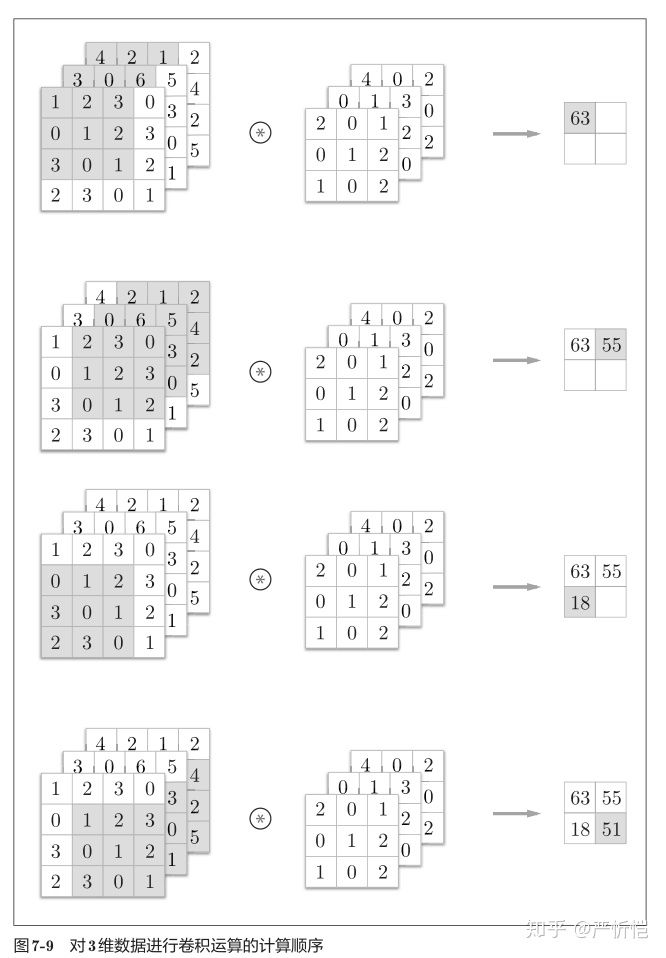
\includegraphics[width=0.90\textwidth]{conv_8}
            \caption{三维卷积运算}
            \label{fig:8}
        \end{figure}
    
        通道方向上有多个特征图时,会按通道进行输入数据和滤波器的卷积运算,并将结果相加,从而得到输出。
        
        将数据和滤波器结合长方体的方块来考虑,3维数据的卷积运算会很容易理解。方块是如图\ref{fig:9}所示的3维长方体。把3维数据表示为多维数组时,书写顺序为$(channel, height, width)$。
        
        \begin{figure}[!htbp]
            \centering
            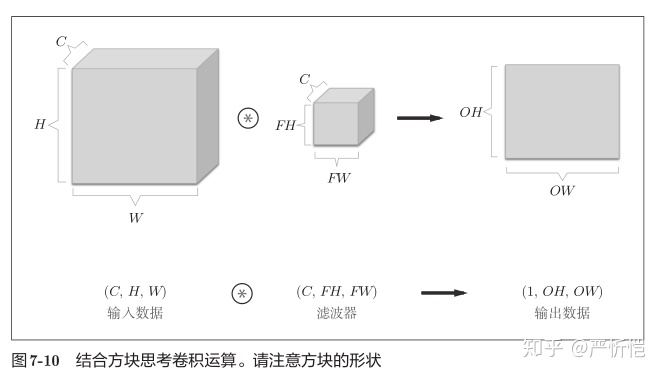
\includegraphics[width=0.90\textwidth]{conv_9}
            \caption{用方块理解三维卷积}
            \label{fig:9}
        \end{figure}
    
        在这个例子中,数据输出是1张特征图。所谓1张特征图,换句话说,就是通道数为1的特征图。那么,如果要在通道方向上也拥有多个卷积运算的输出,该怎么做呢?为此,就需要用到多个滤波器(权重)。用图表示的话,如图\ref{fig:10}所示。
        
        \begin{figure}[!htbp]
            \centering
            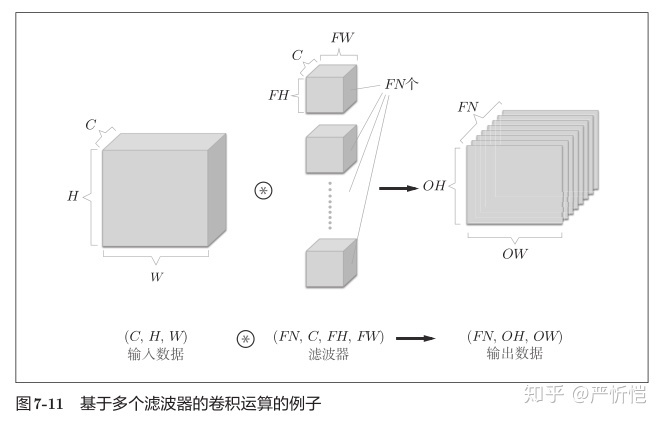
\includegraphics[width=0.90\textwidth]{conv_10}
            \caption{基于多个滤波器的卷积运算}
            \label{fig:10}
        \end{figure}
        
        通过应用FN个滤波器,输出特征图也生成了FN个。如果将这FN个特征图汇集在一起,就得到了形状为$(FN, OH, OW)$的方块。将这个方块传给下一层,就是CNN的处理流。
        
        卷积运算中(和全连接层一样)存在偏置。每个通道只有一个偏置。这里,偏置的形状是$(FN, 1, 1)$,滤波器的输出结果的形状是$(FN, OH, OW)$。这两个方块相加时,要对滤波器的输出结果$(FN, OH, OW)$按通道加上相同的偏置值。
        
            